\subsection{\BaBar/ at PEP-II}
\BaBar/ detector is part of the SLAC facility.
PEP-II $e^- e^+$ collider utilizes PEP-II as the storage ring and SLAC linac as
the injector \cite{Harrison:1998yr}.

% Talk about subdetectors
\BaBar/ is a barrel detector (shown in \autoref{fig:babar_detector_view})
consists of five subdetectors (from inside out):
Silicon Vertex Tracker (SVT) and Drift Chamber (DCH), which measures momentum
and angles of charged particles.
Detector of Internally
Reflected Cerenkov radiation (DIRC), together with SVT and DCH, identifies
charged particles of different masses by Cerenkov ring-imaging and ionization
energy loss of these particles.
Caesium Iodide Electromagnetic Calorimeter (EMC), which measures energy and
position of electromagnetic showers generated by electrons and photons.
A superconducting solenoid with a \SI{1.5}{T} magnetic field surrounding the
EMC, together with Instrumented Flux Return (IFR), is used to identify muons and
some neutral hadrons \cite{Lees:2013uzd}.

\begin{figure}[ht]
    \centering
    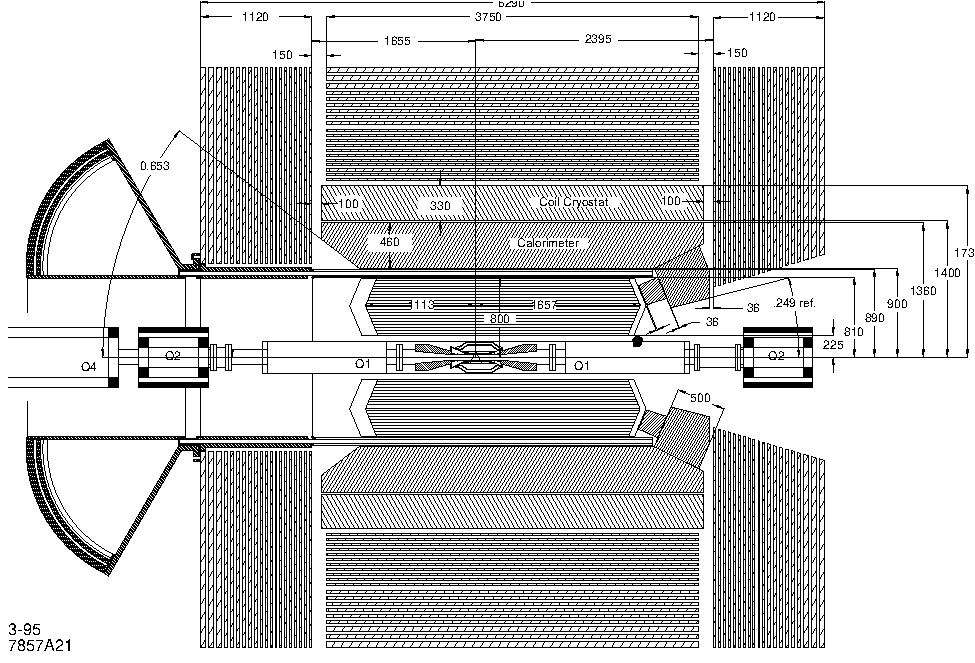
\includegraphics[width=0.7\textwidth]{figs/babar_detector_view.pdf}
    \caption{
        View of the \BaBar/ detector.
    }
    \label{fig:babar_detector_view}
\end{figure}

% Talk about PEP-II and its asymmetrical beam energies
In PEP-II, the $B$ mesons are produced exclusively in the following process:
$e^- e^+ \longrightarrow \Y4S/ \longrightarrow B \overline{B}$.
PEP-II is an asymmetrical accelerator: The $e^-$ beam is boosted to \SI{9}{GeV},
whereas the $e^+$ beam \SI{3.1}{GeV}.
The beam energies are tuned so that the invariant mass is at \Y4S/ resonance;
at the same time, the momentum of the \Y4S/ in the lab frame is
non-zero \cite{Harrison:1998yr}.

This eliminates almost all fragmentation products, reducing combinatorial
background.
Also, since the momenta of $e^- e^+$ is known, several kinematic constraint
can be applied to further suppressing various
backgrounds \cite{Harrison:1998yr}.
Finally, the non-zero momentum of \Y4S/ in the lab frame helps the tracker to
separate the \Y4S/ vertex from the subsequent decay vertices of the $B$ mesons,
which is crucial in calculating the life time of each $B$
meson \cite{McGregor:2008ek}.

% Talk about BaBar being 4 pi
Initial simulation shows that the distribution of angular cross section in the
center of mass frame is ``more symmetric than one might expect"\footnote{
    This is further validated by subsequent measurements.
    See \cite{McGregor:2008ek} for more details.
}, thus the detector needs to cover almost all solid angles
(a $4\pi$ detector) \cite{Boutigny:1995ib}.
Indeed, \BaBar/ has tracking coverage of 0.92, namely 92\% of the $4\pi$ solid
angle \cite{Harrison:1998yr}.

% Talk about tracking
$B$ physics requires excellent vertex resolution and tracking, because the two
$B$ mesons produced by \Y4S/ must be reliably separated.
This translates into a baseline resolution of \SI{80}{\mu m} at
PEP-II \cite{Harrison:1998yr}.
Indeed, \BaBar/'s SVT has a spatial resolution of around \SI{13}{\mu m} at low
angles, and below \SI{30}{\mu m} at higher angles\footnote{
    The angle is measured between beam axial and the momentum direction of the
    $B$ meson.
    For example, if the angle is \ang{0}, then the $B$ meson is flying along the
    beam axial.
    It is expected that the angle will be small.
}
($> \ang{60}$) \cite{Harrison:1998yr}.

% Talk about BaBar's glorious ECAL
% FIXME: Define 'good'.
\BaBar/ has a very good electromagnetic calorimeter:
The EMC is capable to measure photon energies ranging from \SI{20}{MeV} to
\SI{8}{GeV}.
Its energy and angular resolution are given by:
\begin{align*}
    \frac{\sigma_E}{E} &= \frac{(2.30 \pm 0.03 \pm 0.3)\%}{^{4}\sqrt{E}}
    \oplus (1.35 \pm 0.08 \pm 0.2)\% \\
    \sigma_{\theta} = \sigma_{\phi} &= \frac{{4.16 \pm 0.04}~\si{mrad}}
        {\sqrt{E}}
\end{align*}
where $E$ is the numerical part of the energy, measured in
\si{GeV} \cite{Bauer:2005}.
Most \BaBar/ measurements were able to reconstruct charge-neutral particles with
the calorimeter data.

% Talk about luminosity
\BaBar/ collected data from 1999 to 2008. Its integrated luminosity for \Y4S/
reached $424.18 \pm 0.04 \pm 1.82$~\si{fb^{-1}} on-resonance.
This resulted in $(464.8 \pm 2.8) \times 10^6$ $B \overline{B}$
events \cite{Lees:2013rw}.
